%
% File acl2019.tex
%
%% Based on the style files for ACL 2018, NAACL 2018/19, which were
%% Based on the style files for ACL-2015, with some improvements
%%  taken from the NAACL-2016 style
%% Based on the style files for ACL-2014, which were, in turn,
%% based on ACL-2013, ACL-2012, ACL-2011, ACL-2010, ACL-IJCNLP-2009,
%% EACL-2009, IJCNLP-2008...
%% Based on the style files for EACL 2006 by 
%%e.agirre@ehu.es or Sergi.Balari@uab.es
%% and that of ACL 08 by Joakim Nivre and Noah Smith

\documentclass[11pt,a4paper]{article}
\usepackage[hyperref]{report}
\usepackage{times}
\usepackage{latexsym}
\usepackage{graphicx}
\graphicspath{{../figures/}}
\usepackage{url}

\aclfinalcopy % Uncomment this line for the final submission
%\def\aclpaperid{***} %  Enter the acl Paper ID here

%\setlength\titlebox{5cm}
% You can expand the titlebox if you need extra space
% to show all the authors. Please do not make the titlebox
% smaller than 5cm (the original size); we will check this
% in the camera-ready version and ask you to change it back.

\newcommand\BibTeX{B\textsc{ib}\TeX}

\title{Gendered Pronoun Resolution}

\author{Dhruv Patel \\
  IISc, Bangalore \\
  \texttt{dhruvpatel@iisc} \\\And
  Prateek Sachan \\
  IISc, Bangalore \\
  \texttt{prateeksachan@iisc} \\}

\date{}

\begin{document}
\maketitle
\begin{abstract}
  In this project we try solve the problem of Genered  Pronoun Resolution. To train neural networks with less data we show how augmentation can help to reduce overfitting. We have experimented with different architectures including and excluding attention. We observe that attention has no advantage over simple mean. Our model scores 0.2462 (cross entropy) on Kaggle competition, which is better than solution occupying 26th position on the leader board.
\end{abstract}

\section{Introduction and Problem Statement}
Gendered Pronoun Resolution is a subset of co-reference resolution problem. Here we study problem in a setting where we are given a particular male(he, his, him) or female(she, her, hers) pronoun and two candidate nouns in a sentence that match gender of the given pronoun. Task is to figure out which of these two candidates this particular pronoun refers to.  Our architecture can be extended to more than two candidates without any modifications. This problem was posed on Kaggle as a competition by Google AI. Below we show one example sentence of the input. Boldface words are candidate nouns. Underlined noun is correct noun. Italic boldfaced word is the pronoun.
\begin{quote}
   \textbf{\underline{Kathleen}} first appears when \textbf{Theresa} visits \textbf{\textit{her}} in a prison in London.
\end{quote}

\section{Related Work}
Earlier co-reference resolutions approaches using neural networks were proposed by \cite{wiseman2016learning} and \cite{clarkmanning2016deep}. However they used syntactic parsers to hand engineer mention proposal algorithms. Current state-of-the-art model is proposed by \cite{lee2017end}. In their model, they would consider all spans of some maximum length and calculate mention score for that span using a neural network. Than for each span $i$ they would consider all spans $j$ before it and calculate a score for pair $(i, j)$. They also consider special span $\epsilon$ and fix score of $(i, \epsilon)$ to 0. $\epsilon$ span denotes that $i$ is the first co-referent, and nothing before it refers to same entity as $i$.

To find embeddings of spans \citet{lee2017end} used BiLSTM, with GloVe \cite{pennington2014glove} embeddings as input. At the end to calculate fixed size span embedding, they used attention mechanism to find weights and than used weighted combination of embeddings of words in the span. Later \citet{Peters:2018} improved results of this architecture by using ELMo embeddings.

By using transformer network \cite{vaswani2017attention}, \citet{devlin2018bert} have trained BERT model to give contextualized embeddings. These embeddings have got state-of-the-art results in eleven NLP tasks.

\section{Method}
\label{sec:method}
Earlier we started with ambitious goal. Instead of just two candidates, our earlier models used Flair embeddings to find all possible person entities as possible candidates using named entity recognition. However for each sentence we only knew one correct answer. There could have been other entities with some variation to correct name, which we would treat as negative example. It turned out that none of our models worked better with GAP dataset(section \ref{subsec:datasets}). So instead we focused on more simpler setting, where two candidates are given and at most one of them is true. Now our problem was reduced to three class classification.

Our starting point was Lee et al.'s model. First we get BERT embeddings for candidate A, candidate B and a pronoun. We used simple mean to get fixed size vector for each candidate. We have experimented with attention, but in our experiments attention didn't give any significant improvements. In their model they had to find mention score for each span. However in this simpler setting, since candidate spans are given, we modified their architecture to not use mention score. Now we only needed to find two scores, one for each possible candidates.  We pass pair consisting a candidate and a pronoun through three layer fully connected neural network (called scoring function).  We have also experimented with bilinear variation, but that too didn't perform well.  

However, while training we found that, since GAP is a small dataset, our models overfitted. Instead of looking for other datasets with similar characteristics of GAP, we used augmentation. Details of augmentation are explained in section \ref{subsec:augment}. But in summary, each time network sees a sentence, with probability 0.6 it will see random different candidates instead of original candidates. Thus network will have no time to memorize candidates and instead it has to learn other useful features.

\begin{figure}
  \centering
  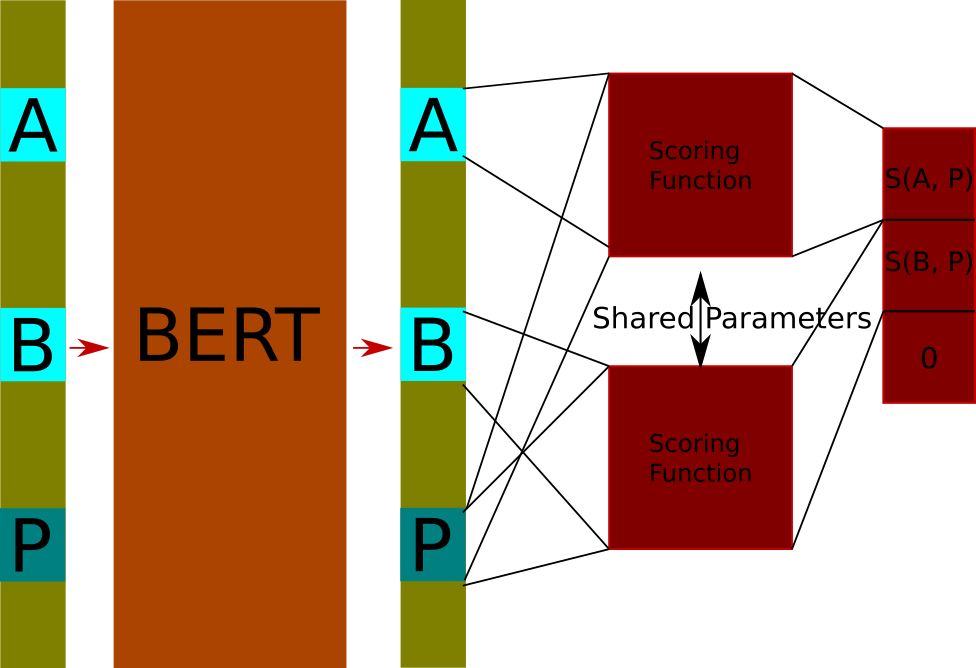
\includegraphics[width=.4\textwidth]{arch.png}
  \caption{Architecture}
  \label{fig:arch}
\end{figure}

Figure \ref{fig:arch} shows our final architecture with respect to which our results are reported in section \ref{sec:results}.
\section{Datasets and Metrics}

\subsection{Datasets}
\label{subsec:datasets}
We have used two datasets in our experiments.
\begin{enumerate}
\item \textbf{GAP} GAP co-reference dataset \cite{webster2018gap} is gender-balanced dataset divided into three sets for development, test and validation. Both development and test sets contain 2000 sentences each. Validation dataset contains 454 sentences. In each sentence there are two possible candidates denoted by A and B respectively. There is one pronoun per sentence. This pronoun can refer to either A or B or neither. 


\item \textbf{DPR} Definite Pronoun Resolution \cite{rahman2012resolving} dataset is divided into two sets for training and testing. There are 1886 sentences in total. Although the original dataset has only one candidate per sentence, there are two sentences having same actors in common(i.e. there are 943 pairs of sentences). So we combined two actors to play as candidates. The resulting dataset is similar to GAP. Below is an example pair.
  \begin{quote}
    \begin{itemize}
    \item James asked \textbf{Robert} for a favor, but \textit{\textbf{he}} refused.
    \item \textbf{James} asked Robert for a favor, but \textit{\textbf{he}} was refused.
    \end{itemize}
  \end{quote}
\end{enumerate}

We have used 2000 sentences from GAP to train, while keeping others aside for validation and test. When we used DPR in addition to GAP, we used both train and test sets of DPR for training. Validation in this case was still done on GAP validation set.

\subsection{Data Augmentation}
\label{subsec:augment}

Earlier we tried our models without any data augmentation. But since GAP has only 2000 sentences in development set, our models overfitted. An SVM trained on these 2000 sentences outperformed neural network architectures that we tried. To compare our later modifications, we will use SVM as a baseline.

To mitigate the situation we applied data augmentation. Our hypothesis is that, since input to our network is just a pair of candidate nouns, it doesn’t matter what these nouns are. If all occurrences of noun `Firstname Lastname’ were to be replaced by some other plausible pair of first name and last names, sentence should make perfect sense. To neural network ``Jon Snow doesn’t know anything.’’ should be similar to ``John Wick doesn’t know anything.’’ 

To augment data we applied simple rule. If both candidate A and candidate B had less than four words then with probability 0.6 we would pick random noun with same number of words. That is if A had three words and B had two words, we would pick alternative A and B with three words and two words respectively. If pronoun is male(female), then only male(female) names are proposed as alternatives. Alternative name for B was chosen such that no word of it was a substring of alternative A. Also none of the alternatives had any overlap with original nouns. Below are the examples of augmented sentences. First sentence is an original, other are augmented. Here Margaret Ray is candidate A and Betsy is candidate B.

\begin{itemize}
\item Tony Markham, a high school senior and the ``Tall Dark Stranger'' \underline{Betsy} fell in love with as a freshman, who has since become a good friend not only to \underline{Betsy} but the entire \underline{Ray} family. \underline{Mrs. Ray}, \underline{Betsy}'s mother. \underline{Mr. Ray}, \underline{Betsy}'s father, who owns a shoestore. \textbf{\underline{Margaret Ray}}, \textbf{\underline{Betsy}}'s sister who is five years younger than she is.
  
\item Tony Markham, a high school senior and the ``Tall Dark Stranger'' \underline{Booth} fell in love with as a freshman, who has since become a good friend not only to \underline{Booth} but the entire \underline{Delgado} family. \underline{Mrs. Delgado}, \underline{Booth}'s mother. \underline{Mr. Delgado}, \underline{Booth}'s father, who owns a shoestore. \underline{Pam Delgado}, \underline{Booth}'s sister who is five years younger than she is.

\item Tony Markham, a high school senior and the ``Tall Dark Stranger'' \underline{Alyssa} fell in love with as a freshman, who has since become a good friend not only to \underline{Alyssa} but the entire \underline{Jolie} family. \underline{Mrs. Jolie}, \underline{Alyssa}'s mother. \underline{Mr. Jolie}, \underline{Alyssa}'s father, who owns a shoestore. \underline{Angelina Jolie}, \underline{Alyssa}'s sister who is five years younger than she is.
\end{itemize}

  
The pool for alternative names was extracted from dataset for stage2 of Kaggle competition. It has around 12K sentences. Figure \ref{fig:augment_dist} shows distribution of names for both genders. One word names are most common in dataset followed by two word names.

\begin{figure}
  \centering
  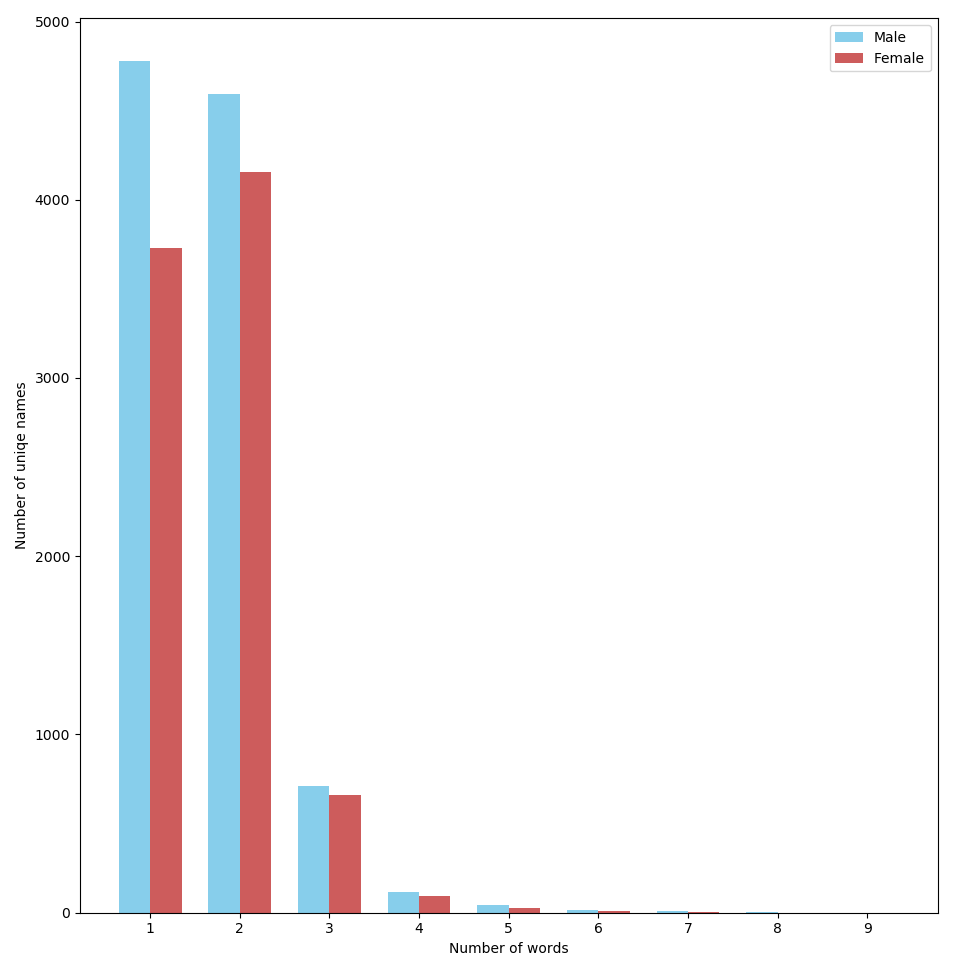
\includegraphics[width=.5\textwidth]{augment_dist.png}
  \caption{Distribution of names.}
  \label{fig:augment_dist}
\end{figure}

\subsection{Metrics}
To compare our results with baseline proposed by \citet{webster2018gap}, we use micro average of F1-scores. To compare our results with other Kaggle competitors, we used cross entropy loss $\mathcal{L}$.

\[
  \mathcal{L} = - \frac{1}{N} \sum_{i=1}^N \sum_{j \in \{A, B, N\}} (y_i^j* log(\sigma(\hat{y_i^j}))).
\]

Where $y_i^j$ is 1 if $j$ is correct candidate for $i^{th}$ example. N denotes neither case. $\hat{y_i^j}$ denotes predicted probability for class $j$ for $i^{th}$ example.

\section{Baselines}
\label{sec:baselines}

\begin{table}
  \centering
  \begin{tabular}{|l|r|r|r|}
    \hline
    & M & F & O \\
    \hline
    Wiseman et al. \shortcite{wiseman2016learning} & 68.4 & 59.9 & 64.2 \\
    Lee et al. \shortcite{lee2017end} & 67.2 & 62.2 & 64.7 \\
    \hline
    SVM-8 & \textbf{77.10} & \textbf{79.10} & \textbf{78.10} \\
    \hline
  \end{tabular}
  \caption{Baselines}
  \label{tab:baselines}
\end{table}


Table \ref{tab:baselines} shows baselines we have used. First three rows were reported by Webster et al.\shortcite{webster2018gap}. \textbf{M} column denotes F1 score for male, same for female and \textbf{O} denotes score for all. However these baseline models were not trained on GAP dataset\footnote{Authors have reported results on development set and not test set. So to be fair, we have trained our models actually on test set and reported results on development set. On Kaggle too published test set was actually development set in Github repository}. For example Lee et al. \shortcite{lee2017end} was trained on onto notes. 

In last row we note the baseline that we established. That score was obtained by SVM trained on $768 \times 3$ dimensional vectors. These vectors were obtained by concatenating outputs of 8th layer BERT(base model) for $A$, $B$ and $P$. Where $P$ denotes a pronoun.  

\section{Experiments}
\label{sec:experiments}

We have ran different experiments. In one set of experiments we varied different layers of BERT base model and BERT large model. There were $24 + 12$ different experiments done. Initially for base model, our best score(cross entropy) was 0.59, which was obtained by 8th layer and scoring function explained in section \ref{sec:method}. This model was unable to pass the baseline that we had established (i.e. SVM). The cross entropy of SVM-8 is 0.51.

Our scoring function is multi layer perceptron with three linear layers with ReLU activation. First layer has 64 units, second layer has 32 units and final layer has one output unit. We pass $[C(V(A))|V(P)]$ and $[C(V(B))|V(P)]$ through this function and obtain scalar score. Here $V(w)$ is an output of certain layer BERT for token $w$. Since BERT uses WordPiece tokenizer, sometimes even one word noun gets tokenized into multiple tokens. $C$ function combines these multiple vectors into single fixed size vector. We have used two different types of $C$. In one case we just take a mean of all these vectors. That is bag of tokens. In other model we learn attention on these tokens and then combine proportional to the attention. We used Multiplicative attention.

We have implemented our models in PyTorch. We used pretrained BERT models from Hugging Face\footnote{https://github.com/huggingface/pytorch-pretrained-BERT}. We used Adam optimizer with default parameters. We used patience value of 20, that is if no improvement in validation loss happened within 20 epochs, we would stop training. Weight decay of 0.001 was used. Dropout value of 0.5 was used. The best results were obtained by 20th layer of BERT large model.

\section{Results}
\label{sec:results}

\begin{table}
  \centering
  \begin{tabular}{|l|r|r|r|}
    \hline
    & M & F & O \\
    \hline
    SVM-8 & 77.10 & 79.10 & 78.10 \\
    \hline
    MLP             & 89.10 &88.00 & 88.55 \\
    MLP-attn         &  89.50 & 88.40 & 88.95 \\
    MLP-dpr           & 88.90 & 88.70 & 88.80 \\
    MLP-dpr-attn    & 90.10 & 87.90 & 89.00 \\
    \hline
  \end{tabular}
  \caption{F1 score Results}
  \label{tab:accuracy}
\end{table}

\begin{table}
  \centering
  \begin{tabular}{|l|r|r|r|r|}
    \hline
    &M & F & O \\
    \hline
    SVM-8          & 0.5127 & 0.5077 & 0.5102 \\
    \hline
    MLP  & 0.2669 & 0.3412 & 0.3041 \\
    MLP-attn   & 0.2828 & 0.3252 & 0.3040 \\
    MLP-dpr      & 0.2752 & 0.3187 & 0.2969 \\
    MLP-dpr-attn & 0.2706 & 0.3367 & 0.3036 \\
    \hline
  \end{tabular}
  \caption{Cross Entropy Loss on stage 1 test set}
  \label{tab:ce1}
\end{table}
\begin{table}
  \centering
  \begin{tabular}{|l|r|}
    \hline
    & O \\
    \hline
    SVM-8          &  0.7809 \\
    \hline
    MLP  & 0.2462 \\
    MLP-attn   & 0.2545 \\
    MLP-dpr      & 0.2727 \\
    MLP-dpr-attn & 0.2517 \\
    \hline
    Kaggle First & 0.1366 \\
    Kaggle 25th & 0.2403 \\
    \hline
  \end{tabular}
  \caption{Cross Entropy Loss on stage 2 test set}
  \label{tab:ce2}
\end{table}

\begin{table}
  \centering
  \begin{tabular}{|l|r|r|r|r|}
    \hline
    &    precision&    recall&  f1-score&    support \\
    \hline
    A&     0.8635&    0.9533&    0.9062&       856\\
    B&     0.9219&    0.8930&    0.9072&       925\\
    Neither&     0.8113&    0.5890&    0.6825&       219\\
    \hline

  \end{tabular}
  \caption{Precision-Recall of MLP}
  \label{tab:precisionrecall}
\end{table}

Table \ref{tab:accuracy} shows results on our models. When model has \texttt{-attn} suffix, model used attention instead of simple mean. When model has \texttt{-dpr} in it's name we have also used DPR dataset in addition to GAP dataset. We can see that there is no discernible difference in overall accuracy. We discuss implications and our hypothesis in section \ref{sec:discussion}.

Table \ref{tab:ce1} shows cross entropy loss on Kaggle test set of stage 1.  Other models are performing better. In this test set there are 2000 examples.

Table \ref{tab:ce2} shows cross entropy loss on Kaggle test set of stage 2. This test set contains around 12K examples. Since correct answers are not in public domain yet, we obtain these results by uploading our results on Kaggle competition page. Here we see that our SVM baseline fails miserably. However other models performs good. For reference we also list results of composition winner and 25th spot to compare our position.

Table \ref{tab:precisionrecall} shows Precision Recall for different classes on MLP model(2nd row in Table \ref{tab:ce1}) on test set for stage 1. It is interesting to note that for class ``Neither'' recall is 0.58, which is too low. That is our model will say, either A or B often, even though neither of them is true. We believe this is due to class imbalance in training set. Assigning different weights to different classes could mitigate this situation, but we haven't tried that aproach yet.

\section{Discussion}
\label{sec:discussion}

\subsection{Difference(or lack of) between attention and mean}
Looking at results in table \ref{tab:ce1}, we don't see discernible difference between attetion mechanism and simple mean mechanism. To analyze further we compared cosine similarity of the vectors generated after both mechanisms. About 23\% vectors from validation set had cosine similarity less than $0.999$. And none of the vectors had cosine similarity less than $0.99$. This implies that the learned attetion was close to uniform. To confirm this,  we mannually analyzed few random attention weights and they were close to uniform. Although We don't know the side effects of WordPiece tokenization, our hypothesis is that, looking at Figure \ref{fig:augment_dist}, most nouns are single word or double word long. Thus resulting tokenization would not be too long either. And so attention has no advantage in this case.

\subsection{Bias}
\label{sec:bias}
Again, looking at table \ref{tab:ce2}, columns \textbf{M} and \textbf{F}, model MLP has most bias, even though it is best performing model on stage 2 testset. We expected there to be more bias in last two models than first two, since they were trained on DPR dataset as well, which has unbalanced pronouns. GAP dataset on the other hand is balanced dataset. We think this bias stems from BERT embeddings and not from the dataset.

\subsection{Fine tuning BERT}
Even after augmentation, we think that it is not a good idea to fine tune BERT on GAP dataset. Although this may reduce bias, we are afraid that model might learn to remember answer by looking at the context. Augmentation happens only on nouns, context doesn't change. So it might be possible to remember answer based on context. Same applies to using RNN before MLP. RNN might remember answer based on context.

\subsection{Extending to more than two candidaets}
\label{subsec:morecandidates}
Although during training we have two candidates, there is nothing stopping us to have more than two candidates during test time. That is since parameters for scoring function in figure \ref{fig:arch} are shared, we can have final vector of arbitrary size. The next step is softmax over this vector. It doesn't matter the dimensions of this vector, softmax essentially selects top scoring element from input vector. However we were unable to combine NER from Flair and our model, since both use different tokenization. To combine, we would have had to make few changes in our preprocessing code as to incorporate different tokenizations.

\section{Future Work}
For test stage 2, many top ranking users on Kaggle actually retrained their model with 4000 sentences. That is they also included test set of stage 1 during training. First task for future would be to train our model on combined dataset and observe the effects.

We believe, once test set for stage 2 becomes available, we can fine-tune BERT model also. Or we can induce BiLSTM inbetween BERT and MLP.

As noted in section \ref{subsec:morecandidates}, it would be intreseting to check our hypothesis that our architecture should work on more than two candidates.

\bibliography{report}
\bibliographystyle{acl_natbib}

\appendix

\end{document}
